\documentclass[
  twoside,
  11pt, a4paper,
  footinclude=true,
  headinclude=true,
  cleardoublepage=empty
]{scrbook}

\usepackage{dissertation}

% ACRONYMS ----------------------------------------

% import the necessary package with some options
%\usepackage[acronym,nonumberlist,nomain]{glossaries}

% enable the following to avoid links from the acronym usage to the list
% \glsdisablehyper

% displays the first use of an acronym in italic
% \defglsdisplayfirst[\acronymtype]{\emph{#1#4}}

% the style of the Glossary
\glossarystyle{listgroup}

% set the name for the acronym entries page
\renewcommand{\glossaryname}{Acronyms}

% better looking urls
\hypersetup{urlcolor=blue}

% here are the acronym entries
\newacronym{mei}{MEI}{Mestrado em Engenharia Informática}
\newacronym{di}{DI}{Departamento de Informática}
\newacronym{um}{UM}{Universidade do Minho}

\newacronym{ai}{AI}{Artificial Intelligence}
\newacronym{ann}{ANN}{Artificial Neural Network}
\newacronym{ml}{ML}{Machine Learning}
\newacronym{dl}{DL}{Deep Learning}
\newacronym{soa}{SOA}{Service Oriented Architecture}
\newacronym{cadx}{CADx}{Computer-Aided Diagnosis}
\newacronym{mlp}{MLP}{Multi Layer Perceptron}
\newacronym{dnn}{DNN}{Deep Neural Networks}
\newacronym{cnn}{CNN}{Convolutional Neural Network}
\newacronym{rnn}{RNN}{Recurrent Neural Network}
\newacronym{lstm}{LSTM}{Long Short-Term Memory Unit}
\newacronym{rbm}{RBM}{Restricted Boltzmann Machine}
\newacronym{dbn}{DBN}{Deep Belief Network}
\newacronym{roi}{ROI}{Region Of Interest}
\newacronym{auc}{AUC}{Area Under the ROC Curve}
\newacronym{svm}{SVM}{Support Vector Machine}
\newacronym{mlo}{MLO}{Medio-Lateral Oblique}
\newacronym{cc}{CC}{Craniocaudal}
% ...

% these could go in an acronyms.tex file, and loaded with:
% \loadglsentries[\acronymtype]{Parts/Definitions/acronyms}
% when using this, you may want to remove 'nomain' from the package options

%% **MORE INFO** %%

%to add the acronyms list add the following where you want to print it:
%\printglossary[type=\acronymtype]
%\clearpage
%\thispagestyle{empty}

%to use an acronym:
%\gls{qps}

% compile the thesis in command line with the following command sequence:
% pdlatex dissertation.tex
% makeglossaries dissertation
% bibtex dissertation
% pdlatex dissertation.tex
% pdlatex dissertation.tex

% -------------------------------------------------

% Title
\titleA{Intelligent Medical Image Analysis}
\titleB{} % (if any)
\subtitleA{A \textit{Deep Learning} approach to breast}
\subtitleB{cancer diagnosis} % (if any)

% Author
\author{João Pedro Pereira Fontes}

% Supervisor(s)
\supervisor{Professor Miguel Angel Guevara Lopez}
\cosupervisor{Professor Luís Gonzaga Mendes Magalhães}

% Date
\date{\myear} % change to text if date is not today

% Glossaries & Acronyms
\makeglossaries
\makeindex[title=Index of Terms]

% Define Acronyms
%\input{sec/acronyms}
%\glsaddall[types={\acronymtype}]

\ummetadata % add metadata to the document (author, publisher, ...)

% Utils
\newcommand{\source}[1]{\vspace{-3pt} \caption*{Source: {#1}} }

\begin{document}
  \pagenumbering{gobble}
  % Cover page ------------------------------------
  \umfrontcover
  \null\newpage
  \umtitlepage

  \begingroup
  \fontsize{12pt}{15pt}\selectfont

  % Add acknowledgements --------------------------
  \chapter*{Acknowledgements}
    % ... Supervisors
    % ...

    % ... Algoriteam
    % ...

    % ... Close Friends
    % ...

    % ... CVIG Group and CCG
    % ...

    % ... University
    % ...

    % ... Family & Girlfriend
    % ...

  \null\newpage\null\newpage
  % Add abstracts (en,pt) -------------------------
  \chapter*{Abstract}
    Once medical images were scanned and uploaded to a computer, researchers began to create automated medical imaging systems. From the 1970's to the 1990's, medical imaging was performed with sequential application of low-level pixel processing and mathematical modeling to solve specific tasks such as organ segmentation. At the end of the 1990's, supervised techniques began to appear, where data extracted from the images were used to train models and classification systems. One example is the use of automated classifiers to build support systems for cancer detection and diagnosis. This pattern recognition and / or Machine Learning approach is still very popular and represented a shift from systems that were completely human-engineered to computer-trained systems with the use of specific (manually drawn) features and automatically extracted from the training data (example). The next step is that the algorithms directly learn the characteristics of the pixels of the images. This is the basic concept of Deep Learning algorithms: multi-layered models that transform input data (images) into outputs (e.g. the presence or absence of pathological lesions or cancer).

    This study intends to present ways of using Deep Learning algorithms in the analysis of medical images, in particular for the classification of pathological lesions representative of breast cancer phenotypes.

    $\\$\textbf{Keywords: } Medical Image Analysis, Deep Learning, Artificial Intelligence, Breast Cancer Diagnosis

  \null\newpage\null\newpage
  \chapter*{Resumo}
    Assim que foi possível digitalizar e carregar imagens médicas num computador, os investigadores começaram a criar sistemas automatizados para análise de imagens médicas. No intervalo dos anos 70 até aos anos 90, a análise de imagens médicas foi feita com a aplicação sequencial de processamento de pixeis de baixo nível e modelação matemática para resolver tarefas específicas como, por exemplo, a segmentação de órgãos. No final dos anos 90, começam a aparecer as técnicas supervisionadas, onde os dados extraídos das imagens são usados para treinar modelos e sistemas de classificação. Um exemplo é o uso de classificadores automáticos para construir sistemas de apoio à deteção e diagnóstico do cancro. Esta abordagem de reconhecimento de padrões e/ou Machine Learning\index{Machine Learning} ainda é muito popular e representou uma mudança nos sistemas que eram completamente projetados por seres humanos para sistemas treinados por computadores com recurso ao uso de características específicas (manualmente desenhadas) e extraídas automaticamente dos dados de treino (exemplo). O passo seguinte a alcançar é que os algoritmos aprendam directamente as características dos pixeis das imagens. É este o conceito base dos algoritmos de Deep Learning: modelos (redes) compostos por muitas camadas que transformam dados de entrada (imagens) em saídas (por exemplo, a presença ou ausência de lesões patológicas ou cancro).

    Pretende-se com este estudo apresentar formas de usar algoritmos de Deep Learning na análise de imagens médicas, em particular para a classificação de lesões patológicas representativas de fenotipos de cancro da mama.

    $\\$\textbf{Palavras-Chave: } Análise de Imagem Médica, Deep Learning, Inteligência Artificial, Diagnóstico de Cancro da Mama

  % Summary Lists ---------------------------------
  \tableofcontents
  \listoffigures
  \listoftables
  \printglossary[title=Acronyms, toctitle=List of terms]
  \clearpage
  \pagestyle{plain}

  \pagenumbering{arabic}

  % CHAPTER - Introduction ------------------------
  \chapter{Introduction} \label{intro}
    % ... Intro's intro
    Since computers first came up and started to replace humans in many tasks, the evolution of these techniques follows an exponential growth that presently is giving us the power to came up with results to solve our problems much more quickly and, very often, more accurately than only with human effort. This is possible with the use of \gls{ai}. \gls{ai} algorithms can now provide an environment in which computers can learn from training data and provide results that are more like those provided by a human.

    % ... What is AI?
    \gls{ai} is a branch of computer science that seeks to make computers have human-like behaviors, like think, react and learn \cite{russell2010artificial}. These actions allow computers to solve problems that are normally associated with cognitive functions and that usually require some level of training to be solved.   % ...

    % ... Machine Learning
    Ever since \gls{ai} is studied, one of the areas that gained a major role in this study is \gls{ml}. Machine Learning\index{Machine Learning} is a science that studies the ways that a computer can solve a problem without being explicitly programmed to do so or, in other words, to improve with experience \cite{carbonell1983overview}. To do this, the computer learns from a training set of data and adjusts itself to fit the results that are expected to be produced. The process of learning follows a technique that tries to minimize an error metric and, as a result, to maximize the algorithm's performance in responding to the questions asked.
    With this, it is possible to bring computers closer to perform tasks that until now were only possible to perform by humans, such as recognizing an image, video, sounds, etc. % ...

    % ... Some Applications of Machine Learning
    With the introduction of Machine Learning, fields like Computer Vision and Natural Language Processing got a huge boost in its performance. Previous algorithms in these fields of study had a high complexity and required many resources in order to be able to provide results in a short time. Introducing Machine Learning, the algorithms have shifted the main workload to the training stage, releasing the classification stage (recognition) from this task. With this, it is possible to provide results faster than using traditional techniques, although it may have a lower degree of confidence, which depends on the algorithm's training.

    % ... New Approaches to Machine Learning: Deep Learning
    Although Machine Learning\index{Machine Learning} algorithms produced very satisfactory results, there was a ceiling in the performance that these algorithms could not overpass and that delayed the developments of this area for some years. With the new developments in technology (i.e. the introduction of faster CPUs and GPUs) and the development of new \gls{ann} algorithms, Machine Learning\index{Machine Learning} techniques gained a new breath and, with the introduction of new approaches like \gls{dl}, could overcome the ceiling that was imposed before and gave the results that were expected some years before. As we can see in figure \ref{intro:fig:deep-learning-performance}, the difference between modern Deep Learning\index{Deep Learning} and older Machine Learning\index{Machine Learning} algorithms performance is huge when the amount of data is increased.

    \afterpage{
      \begin{figure}[t]
        \centering
        \includegraphics[width=.6\textwidth]{"./img/deep-learning-performance"}
        \caption[Deep Learning vs. Traditional Machine Learning]{Deep Learning\index{Deep Learning} performance compared to traditional Machine Learning\index{Machine Learning} algorithms. When the amount of data increases, traditional Machine Learning methods are not able to take advantage of that amount, stabilizing its performance in a ceiling. However, Deep Learning\index{Deep Learning} methods learn better with more data, being able to perform significantly better than traditional methods do.\\
        Source.: \href{http://bit.ly/2E6Iofb}{http://bit.ly/2E6Iofb}, Accessed 02 November 2017}
        \label{intro:fig:deep-learning-performance}
      \end{figure}
    }

    This new breath in Machine Learning \index{Machine Learning} algorithms given by the introduction of \gls{soa} Deep Learning \index{Deep Learning} models in the field of medical image analysis is the object of study of this dissertation. In specific, we aim to explore \gls{dl} methods for breast cancer diagnosis. Deep Learning\index{Deep Learning}-based models have demonstrated to be successful in identifying and classifying pathological lesions in several medical imaging modalities (e.g. X-ray, PET-CT, ultrasound and MRI)

    \section{Breast Cancer Diagnosis} \label{intro:case-study}
      % ... A Basic Definition
      According to the NCI\footnote{National Cancer Institute \href{https://www.cancer.gov/types/breast}{https://www.cancer.gov/types/breast}, Accessed 04 November 2017} Dictionary of Cancer Terms, Breast Cancer is a malign tumor that forms in breast tissue. Like any other cancer, cells become more and more abnormal, old or damaged cells survive when they should die, and new cells form when they are not needed. These extra cells can divide without stopping and may form growths called tumors. This originates a set of symptoms that may cause death to the person suffering from this disease if not treated well and as soon as possible. Breast cancer usually occurs in women, although it can also appear in men more rarely.

      % ... Brest Cancer Statistics
      Breast cancer is one of the most spread chronic non-communicable diseases in the world. According to the American Cancer Society \cite{american2015global}, breast cancer represents 25 percent of the new cancer diagnostics in women worldwide, being the greatest cause of death in world's developing regions.

      % ... Problem Presentation
      Having this in mind, the purpose of this dissertation is to introduce Deep Learning\index{Deep Learning} functionalities to improve the current \gls{cadx} methods of breast cancer diagnosis. Current \gls{cadx} methods already help medical professionals in their diagnostic tasks, improving diagnosis accuracy and achieving a earlier diagnosis, which gives a bigger change of recovery to patients. Having such a huge role in diagnosis, \gls{cadx} methods need to be improved in order to achieve a better performance in classifying cancer phenotypes. Since current \gls{cadx} methods use Machine Learning\index{Machine Learning} algorithms in their tasks, the introduction of Deep Learning\index{Deep Learning} can give a boost in these methods performance.

    \section{Motivation and Main Aims} \label{intro:objectives}
      % ... Motivation
      This work has its motivation based in the statistics presented on section \ref{intro:case-study}. Watching the numbers being so large worldwide, it is necessary to provide better methods to help medical professionals in their diagnostic activities. Achieving an earlier and more accurate diagnosis will make the mortality numbers come down, helping to save more lives. The introduction of \gls{cadx} systems can bring improvements in the early cancer detection process. With this, the main aims of this work are:

      \begin{itemize}
        \item To carry out a study of the algorithms and tools of Deep Learning\index{Deep Learning} , in specific for analysis of medical images;
        \item Implement selected Deep Learning\index{Deep Learning} algorithms on high-performance computing infrastructures (GRID, Cloud);
        \item Test the algorithms with higher performance in a benchmarking dataset of images of patients with breast cancer.
      \end{itemize}

    \section{Document Structure} \label{intro:organization}
      This dissertation is organized in \begin{NoHyper}\ref{conclusion}\end{NoHyper} chapters that describe the application area and present a solution to the problem of diagnosing breast cancer using Deep Learning\index{Deep Learning} .

      % ... Introduction
      Chapter \ref{intro} presents the topic of study and provides the motivation and main aims that lead to this work.

      % ... State of the Art
      Chapter \ref{background} provides some background and context to this work, by presenting the current state of the art of Deep Learning\index{Deep Learning}, including some of the most used methods and structures. It also adds some related work in the Deep Learning\index{Deep Learning} thematic, presenting some of its applications. Finally, it provides a survey on medical image analysis, showing the current applications and how could Deep Learning\index{Deep Learning} be helpful in this area.

      % ... Problem Presentation and Proposed Approach to Solution
      Chapter \ref{problem} presents the problem treated in this dissertation, showing some existing approaches. It also describes the design and architecture of the proposed approach by this work.

      % ... Development
      Chapter \ref{development} shows all details of implementation of our proposed approach, including the decisions made and the performance improving strategies, throughout the details of implementation in a high performance environment, and the outcomes presented to this work.

      % ... Results
      Chapter \ref{experiments} presents a proof of concept of this work, by showing the tests made on this solution.

      % ... Conclusion
      Finally, chapter \ref{conclusion} concludes this dissertation and presents prospects for future work.

  % CHAPTER - State of the Art --------------------
  \chapter{Background} \label{background}
    This chapter provides some context to the work presented in this dissertation. Having this, this chapter is centered in presenting the concepts of Medical Image Analysis, with an emphasis in breast cancer diagnosis. It also presents the concepts behind Deep Learning\index{Deep Learning}, since its origins in Machine Learning, the current state of the art and, finally, how it can be used to build \gls{cadx} systems. It also presents

    \section{Machine Learning Basics} \label{background:machine-learning}
      % ... Some Definitions
      Machine Learning\index{Machine Learning} is a field of computer science that studies and tries to implement learning capabilities, like humans possess, into computers. Learning capabilities on computers can be defined as \cite{mitchell1997machine}: "A computer program is said to learn from experience E with respect to some class of tasks T and performance measure P if its performance at tasks in T, as measured by P, improves with experience E.". In this definition we can find the concepts like \textit{experience}, \textit{class of tasks} and \textit{performance measure}, that help understand what Machine Learning\index{Machine Learning} really is. Machine Learning\index{Machine Learning} algorithms try to improve its performance in a set of \textit{tasks} with training (the act of building \textit{experience}), in order to decrease the value of an error metric (used to \textit{measure performance}). The lower is this error metric, the better is the performance of the algorithms. Machine Learning\index{Machine Learning} methods are generally separated into two different groups:

      \begin{itemize}
        \item \textit{Supervised methods} - in these methods, algorithms are trained using a dataset that already answers to the questions asked. In other words, all the instances have a label that corresponds to the answer that has to be given for this class (category) of instances. This label is used for the algorithm to adjust itself to giving the right answer to the question asked. Examples of these methods are classification and regression methods;
        \item \textit{Unsupervised methods} - unlike supervised methods, these strategies try to deduce the label that accompanies the records in supervised methods. These methods are useful to find patterns in data and when we don't have an annotated dataset to train a supervised model, to infer the classes for each record. Clustering methods are examples of these methods.
      \end{itemize}

      \subsection{Neural Networks}
        Neural networks are Machine Learning\index{Machine Learning} algorithms that are inspired by the human brain structure. It forms the basis in major Deep Learning\index{Deep Learning} methods. These models are composed of neurons, that have activation functions and weights. Neurons are connected to each other, where the output of some neurons is the input of other(s), giving the model a network shape, like it is seen in figure \ref{background:machine-learning:structure}.

        \afterpage{
          \begin{figure}[t]
            \centering
            \def\layersep{3cm}
            \includegraphics[width=0.75\textwidth]{"./img/neural-net-structure"}
            \caption[Structure of a standard artificial neural network]{Structure of a standard \gls{ann}. Computation starts in the input layer, passing through hidden layers and ending in the output layer. This results in a feed-forward architecture, where connections never form a cycle.\\
            Source.: \href{http://bit.ly/2EkesLZ}{http://bit.ly/2EkesLZ}, Accessed 14 November 2017}
            \label{background:machine-learning:structure}
          \end{figure}
        }

        \paragraph{Weights}
          Basic training of neural networks will give the input connections of a neuron different weights, modifying the output value of a neuron. After this training phase, these weights will give a bigger role to more important connections. With this, the input value of a connection will be multiplied by the connection's weight. All values from input connections will be integrated and reduced to a single value (usually all values are summed). Additionally, it can be introduced a value (+1) called \textit{bias}, that ensures that certain conditions are established for each node. Giving input values, the network will produce an output label (e.g. class) based on its training.

        \paragraph{Activation}
          When input arrives at the neuron, it is computed based on the weights and bias and an output value is calculated, also called the neuron activation. This activation will be the value outputted to all the neuron's connections. To produce this output, a transfer function is used to limit the output range and to introduce a non-linear component in the output value, usually giving the network the capacity to approximate any function \cite{leshno1993multilayer}. The most used transfer functions are softmax, hyperbolic tangent (tanh) or sigmoid. It is usual that transfer functions give an output in the interval $[0,1]$, but uses of functions with intervals $[-1,1]$ and even $[-\infty,+\infty]$ have proven to give good results in certain cases \cite{karlik2011performance}.

          Therefore, in order to get the output $\boldsymbol{y}$ of a neuron $n$, with input $\boldsymbol{x}$:

          \begin{equation}
            \boldsymbol{y}\ =\ \sigma\ (\boldsymbol{W}_n\boldsymbol{x}\ +\ \boldsymbol{b})
          \end{equation}

          where $\boldsymbol{W}$ represents the weights, $\sigma$ the activation/transfer function and $\boldsymbol{b}$ the bias. Therefore, using a neural network with multiple layers, also called \gls{mlp}, the function computed in a neuron on layer $n$ can be described by:

          \begin{equation}
            f\ (\boldsymbol{x,W,B})\ =\ \sigma\ (\boldsymbol{W}_n\ \sigma\ (\boldsymbol{W}_{n-1}\ ...\ \sigma\ (\boldsymbol{W}_0\ +\ \boldsymbol{B}_0)\ ...\ +\ \boldsymbol{B}_{n-1})\ +\ \boldsymbol{B}_n)
          \end{equation}

          where $\boldsymbol{B}$ represents the bias values for all neurons.

        \afterpage{
          \begin{figure}[t]
            \centering
            \includegraphics[width=.75\textwidth]{"./img/node-structure"}
            \caption[Illustration of a neural network's neuron structure]{Illustration of a neural network's neuron structure. When input $\boldsymbol{x}_n$ arrives to the neuron, it is multiplied by the connection's weight $\boldsymbol{w}_n$ and finally integrated with the rest of the input values, using the summation function. After the bias $\boldsymbol{b}_k$ is added, the resulting value $\boldsymbol{v}_k$ is passed to the activation/transfer function $\boldsymbol{\phi}$, producing output $\boldsymbol{y}_k$\\
            Source.: \href{http://bit.ly/2AErAcp}{http://bit.ly/2AErAcp}, Accessed 15 November 2017}
            \label{background:machine-learning:node-structure}
          \end{figure}
        }

        \paragraph{Back-propagation}
          % ... Some Definitions
          Neural networks, like all Machine Learning\index{Machine Learning} methods, learn with experience. During its training phase, the system must be fitted in order to overcome the error generated in a prediction. The most used technique in network training is the back-propagation algorithm \cite{rumelhart1988backpropagating}. This algorithm propagates the error backward, updating connection weights based on the error value for each iteration. It starts on the output layer and goes all the way to the input layer, searching for the minimum in the error function. It is based on the Gradient Descent technique, using a learning rate to give bigger or smaller steps in its iterations. A high learning rate will learn very quickly but it may cause the error not achieving a minimum. On the other hand, a low learning rate will be to slow and it will take a large number of epochs (iterations on the training dataset) to learn all the data. The perfect learning rate is a half-term between these two, giving the neural network the capacity to produce generalized predictions without the possibility to overfit the training set. The performance evolution during the training phase for both the training and validation sets can be seen in figure \ref{background:machine-learning:back-propagation}.

        \afterpage{
          \begin{figure}[t]
            \centering
            \includegraphics[width=.75\textwidth]{"./img/training"}
            \caption[Neural Networks error evolution in training]{Example of error evolution in a neural network training. Increasing the number of training iterations will result in a better performance in evaluating the training set. The perfect value of learning epochs is when the error when evaluating the validation data starts increasing, which gives the indication that the neural network is beginning to over-fit the training data \cite{dayhoff2001artificial}, losing its capacity to generalize to other data other than the training one. \\
            Source.: \href{http://bit.ly/2D3wnXB}{http://bit.ly/2D3wnXB}, Accessed 21 November 2017}
            \label{background:machine-learning:back-propagation}
          \end{figure}
        }

    \section{Medical Image Analysis} \label{background:medical-image}
      % ... Some Definitions
      Medical Image Analysis is a sub-field of computer vision that concerns with knowledge extraction from medical images/exams like X-ray, ultrasound or MRI \cite{dhawan2011medical}. After obtaining these images, computers analyze them in order to determine the presence or absence of lesions, only visible through the use of risky surgical interventions.

      % ... Evolution
      The process of analyzing these images began to be done only by experts, who would determine the existence or absence of these lesions through the visual analysis of the images obtained. With the advance of technology, medical image analysis through computer become an aid to specialists, since it facilitated diagnostic processes using computer vision algorithms to make certain processes easier, such as organ segmentation \cite{karssemeijer1988recognition, punia2013review} or lesion classification \cite{wolberg1994machine} . With the advent of machine learning algorithms, it was possible to teach the machines how to diagnose based on features extracted from the images obtained by medical imaging. By using variety-rich datasets, covering a significant number of possible cases, it would be possible to obtain good diagnostic results. An example proposed by López et al. in 2007 \cite{lopez2007breast} was to identify cases of breast cancer using machine learning tools.

      % ... Use of Deep Learning
      As was the norm for traditional machine learning algorithms, they reached a point where it was not possible to obtain better results than the ones obtained at the time, already shown in previous sections. With this, Deep Learning became the first aim in research in medical image analysis. As already reported in section \ref{background:deep-learning}, Deep Learning algorithms can learn features directly from raw data (e.g. image pixels), so the intervention of an expert for handcrafted feature extraction is no longer necessary for the algorithms to do its job. These algorithms can achieve a better performance than traditional machine learning techniques, which will lead to better results in diagnostic and to the salvation of many lives.

      \paragraph{Classification}
        Most Deep Learning approaches to medical image analysis tend to classification tasks. In here, one can find examples like image/exam classification (using the whole image, the output will be the existence or not of, e.g. a disease) or lesion classification (using an image, it will assign a class into parts of the image, giving a single image multiple classes).

      \paragraph{Segmentation}
        Another task with great importance in medical image analysis where Deep Learning techniques are used is segmentation. In here, organ, subsection or lesion segmentation are the major areas of research. Using segmentation in diagnosis, the expert's work will be facilitated be the visual feedback created by the segmetation process. An example of brain matter and fluids segmentation is presented in figure \ref{background:medical-image:segmentation}.

        \begin{figure}[t]
          \centering
          \includegraphics[width=0.65\textwidth]{"./img/img-classification-segmentation"}
          \caption[Example of brain subsections segmentation]{Example of brain subsections segmentation. This image shows the original exam (CT-scan), the individual segments captured by the segmentation algorithm and the final segmented image using different colors.
          \\Source.: \href{http://bit.ly/2CClqv3}{http://bit.ly/2CClqv3}, Accessed 6 January 2017}
          \label{background:medical-image:segmentation}
        \end{figure}

      \subsection{Breast Cancer Diagnosis} \label{background:medical-image:breast-cancer-diagnosis}
        Breast cancer diagnosis is one of the main topics in medical image analysis research nowadays. Since breast cancer is one of the most spreaded and deadly diseases in the world, researchers try to find new ways of diagnosing it sooner and accurately.

        The most common types of breast cancer start in the ducts that carry milk to the nipple or in the glands that produce the milk. These cancers are called ductal and lobular cancers respectively \cite{hunt2012diseases}. These tumors can form a lump in the breast tissue that is visible in breast exams like mammography/mammogram or MRI.

        \afterpage{
            \begin{figure}[t]
                \centering
                \begin{subfigure}[t]{0.5\textwidth}
                  \centering
                  \includegraphics[width=\linewidth]{"./img/ductal-cancer"}
                  \caption{Ductal Ductal Cancer}
                  \label{background:medical-image:breast-cancer-diagnosis:ductal}
                \end{subfigure}%
                \begin{subfigure}[t]{0.5\textwidth}
                  \centering
                  \includegraphics[width=\linewidth]{"./img/lobular-cancer"}
                  \caption{Lobular Breast Cancer}
                  \label{background:medical-image:breast-cancer-diagnosis:lobular}
                \end{subfigure}
                \caption[Schemes for Ductal and Lobular Breast Carcinomas]{Schemes for Ductal and Lobular Breast Carcinomas. Ductal Tumors form in the ducts that carry milk to the nipple. In the case of Lobular Tumors, they form in the breast lobules, the structures responsible for producing milk.\\Source.: \href{http://bit.ly/2DgnkFg}{http://bit.ly/2DgnkFg}, Accessed 11 Jan 2018}
                \label{background:medical-image:breast-cancer-diagnosis:types}
            \end{figure}
        }

        % ... Diagnostic Systems
        \paragraph{Mammography/Mammogram}
          Mammography is a method for breast cancer screening that uses X-rays to get a X-ray film of the breast \cite{starting2012mammography}. This exam is the oldest in breast examining and is the primary exam for cancer detection. Some advances have been made in the late years that include:

          \begin{itemize}
            \item Digital Mammography - also called full film mammography, is a method that converts X-rays into mammographic pictures, producing a digital image that can be used in \gls{cadx} systems without scanning. this method produces less error that the scanning of X-ray films;
            \item Breast Tomosynthesis - also called 3D mammography, is a method where multiple images are retrieved from the breast, using different angles to produce a 3D model after reconstruction.
          \end{itemize}

          These methods can be used by \gls{cadx} systems to search for abnormal areas in the breast (e.g. abnormal masses) that could indicate cancer. \gls{cadx} systems nowadays use primarily film and digital mammographies, although tomosynthesis is starting to appear in breast cancer research. Some of the uses of these exams are presented in section \ref{problem:approaches}.

    \section{Deep Learning} \label{background:deep-learning}
      % ... Some Definitions
      When traditional Machine Learning\index{Machine Learning} methods reached its performance ceiling, Deep Learning\index{Deep Learning} techniques appeared. Deep Learning\index{Deep Learning} is just an extension of Machine Learning\index{Machine Learning} methods, where the algorithms learn the true representation and features of data by itself, without being programmed or informed of which features to extract \cite{lecun2015deep}. With this, Deep Learning\index{Deep Learning} methods can be fed with raw data (e.g image pixels) and automatically discover the correct features to extract and train itself based on those features.

      % ... Evolution
      Major Deep Learning\index{Deep Learning} techniques are based on \gls{dnn}, an extension of traditional feed-forward artificial neural networks that present multiple hidden layers. Having a more complex structure, it will take more time to train these networks, although it will have a greater capability of learning. With a greater number of hidden layers, the input data is decomposed into simple data, allowing the network to learn more complex features and representations, acquiring a great generalization capability. The great complexity of this structures made them impractical to be used without an hardware acceleration. With the introduction of GPU computation, \glspl{dnn} gained a huge boost in its training, which allowed them to be tested and improved. The most popular \gls{dnn} approaches are \glspl{cnn} and \glspl{rnn}, being these architectures the most widely used in image analysis. The following sections present some details about the most used Deep Learning\index{Deep Learning} methods.

      \subsection{Convolutional Neural Networks} \label{background:deep-learning:cnn}
        % ... Some Definitions
        \glspl{cnn} are a \gls{dnn} variant very useful in image analysis, being able to use convolution and pooling layers to extract features from the input images. Convolution layers will apply filters to extract features and pooling layers will highlight these features, increasing the level of the input to the next layer. After the feature extraction phase, the network uses fully-connected layers (i.e. simple feed-forward neural networks layers) that will perform the classification tasks based on the features extracted by the convolutional and pooling layers. % ...

        \afterpage{
          \begin{figure}[t]
            \centering
            \includegraphics[width=.99\textwidth]{"./img/cnn-architecture"}
            \caption[Example of a CNN architecture]{Example of a \gls{cnn} architecture. Given an input image, the \gls{cnn} will output the probabilities that the input belongs to each of the classes trained by the model. In this model, the convolutional and pooling layers represent the feature extraction phase and the fully connected layers represent the classification phase.\\
            Source.: \href{http://bit.ly/2CRmiQ3}{http://bit.ly/2CRmiQ3}, Accessed 2 December 2017}
            \label{background:deep-learning:cnn:architecture}
          \end{figure}
        }

        % ... Famous Architectures
        Some \gls{cnn} architectures have become widely used and became references in the Deep Learning\index{Deep Learning} world. LeNet \cite{lecun1998gradient} consisted in an architecture with 2 convolutional layers that was well used in digit recognition. AlexNet \cite{krizhevsky2012imagenet} was very similar to LeNet, but introduced the ReLU function as the neurons' activation function instead of hyperbolic tangent or sigmoid functions, being now the most common function used in \glspl{cnn}. This architecture won the ImageNet ILSVRC challenge in 2012\footnote{See details about the 2012 ImageNet ILSVRC challenge \href{http://www.image-net.org/challenges/LSVRC/2012/}{here}}.
        GoogLeNet \cite{simonyan2014very} was another architecture that become famous after winning the 2014 ImageNet ILSVRC challenge\footnote{See details about the 2014 ImageNet ILSVRC challenge \href{http://www.image-net.org/challenges/LSVRC/2014/}{here}}. This architecture introduced an inception module, that caused the parameters in the network from $60$M (in AlexNet) to 4M, reducing the usage of computation resources.

        \paragraph{Segmentation}
          % ... Some Definitions
          One of the most used applications of \glspl{cnn} is segmentation in an image. It is one of the largely used applications in medical image analysis, in order for computer programs to be able to divide organs in an image. This is achieved by analyzing every pixel in the image and labeling it. The networks used in these tasks apply all the feature extraction filters like normal \glspl{cnn}, but don't have the usual fully-connected layers for the classification phase at the end of the computation. Having only convolutional layers in its architecture, these networks are called Fully Convolutional Neural Networks. An example of segmentation using these networks can be seen here \cite{long2015fully}.

        \paragraph{3D Generalization}
          % ... Some Definitions
          Although \glspl{cnn} where made for 2D image analysis, the convolution process can be generalized for 3D. Instead of using filters in two dimensions, it is used a 3D version of convolution filters.
          These networks are useful in cases like video analysis \cite{ji20133d,diba2016efficient}, 3D object recognition \cite{maturana2015voxnet,socher2012convolutional,huang2016point} or 3D image segmentation \cite{kamnitsas2017efficient}.

          % ...
          % ...

      \subsection{Recurrent Neural Networks}
        % ... Some Definitions
        Recurrent neural networks are a network architecture where we can find direct cycles in its connections. These cycles allow these networks to have a characteristic that differentiates them from regular networks - memory. This characteristic comes because of the fact that past experiences and values influence computing. The value from past experiences is stored in nodes and is stored for the next computation. This characteristic is useful when analyzing data inserted in a time series, that has a correlation in time. So, in order to calculate a certain neuron state $\boldsymbol{y}$ at time $t$, the value from time $t$-1 needs to be used alongside the input value $\boldsymbol{x}$ on time $t$:

        \begin{equation}
            \boldsymbol{y}_t\ =\ \sigma\ (\boldsymbol{Wx}_t\ +\ \boldsymbol{Ry}_{t-1}\ +\ \boldsymbol{b})
        \end{equation}

        where $\boldsymbol{W}$ and $\boldsymbol{R}$ represent the weights and $\boldsymbol{b}$ the bias.

        Since \glspl{rnn} analyze time sequences, these networks need an extension of the back-propagation algorithm in order to link all time steps. This extension is called Back-Propagation Through Time. This algorithm, adjusts the weights using a gradient descent rule, like normal back-propagation does, but it relies in past . Since this rule relies on multiplications, and since \glspl{rnn} use a great number of this operations, the gradients tend to vanish (to become zero), not allowing the network to learn. This problem is called the Vanishing Gradients Problem \cite{hochreiter1998vanishing}. This problem emerged as one great obstacle in \glspl{rnn} performance, only solved later by the introduction of \glspl{lstm}.

        \paragraph{Long Short-Term Memory Units}
          % ... Some Definitions
          \glspl{lstm} are a \gls{rnn} variation that came in the 1990's \cite{hochreiter1997long} to solve the vanishing gradient problem by using a more constant error value, not allowing abrupt changes in it. By preserving the error, these networks can link the time series occurrences in a more efficient way, being well suited for classification tasks. The error is preserved because of the use of a memory cell and three gates: input, output and forget. The cell will store values from previous computations. The input gate will control what value will flow to the network. The forget will control the values that will be stored in the network. The output gate will control what value will be used to calculate the neuron's (considering a \gls{lstm} block a single neuron) activation. This workflow can be seen in figure \ref{background:deep-learning:rnn:lstm:architecture}

          \afterpage{
            \begin{figure}[t]
              \centering
              \includegraphics[width=0.6\textwidth]{"./img/lstm-architecture"}
              \caption[Standard LSTM architecture]{Standard \gls{lstm} architecture. Input $\boldsymbol{X}_t$ flows into the cell and the gates, along with the value stored from last computation. The input cell will determine first which value will be passed to the cell, where the forget gate will control the amount of past information that will erased from memory. Finally, the output gate will determine the final value that will be outputted by the \gls{lstm} block.\\Source.: \href{http://bit.ly/2EkmOD0}{http://bit.ly/2EkmOD0}, Accessed 16 December 2017}
              \label{background:deep-learning:rnn:lstm:architecture}
            \end{figure}
          }

      \subsection{Unsupervised Techniques}
        % ... Some Definitions
        Deep Learning\index{Deep Learning} techniques work better with more data. Using supervised techniques, with more data, comes a great outcome. All the data needs to be labeled so that the algorithm can learn using the answers provided. Having millions of records to label, the work becomes expensive. To overcome this obstacle, unsupervised techniques were created, so that the algorithms could learn from unlabeled data. These algorithms can also be used to create labels in a dataset when they don't exist, in order to provide the labeled dataset to a supervised technique after that process. The following section provide some details about some of the most used unsupervised Deep Learning\index{Deep Learning} techniques like Restricted Boltzmann Machines, Deep Belief Networks and Auto-Encoders.

        \paragraph{Restricted Boltzmann Machines and Deep Belief Networks}
          % ... Some Definitions
          Boltzmann Machines are stochastic \glspl{rnn} and an example of Markov Random Fields \cite{rozanov1982markov} that can fit to a probability function. These networks are composed of two groups of units, visible and hidden units, connected between each other bidirectionally. Since this architecture could result in a great complexity, \glspl{rbm} where created. These networks do not allow connections in-layer, i.e. between units in the same layer. An example of this architecture can be seen in figure \ref{background:deep-learning:rnn:rbm:architecture}. Each node in a visible unit will receive a feature to learn (a pixel value in the case of an image), and pass that value to the next layer, multiplied ny the connection's weight. In the hidden layer, hidden units have associated a bias value, that will be added to the sum of the inputs received from the visible units. The final value goes through the activation function, producing the final output of that unit. So, with input $x$, output $y_t$ of unit $t$ will be:

          \begin{equation}
            y_t = \sigma(\boldsymbol{W} x + \boldsymbol{b})
          \end{equation}

          where $\boldsymbol{W}$ represents the weights, $\boldsymbol{b}$ the hidden unit's bias and $\sigma$ the activation function.

          \afterpage{
            \begin{figure}
              \centering
              \includegraphics[width=0.65\textwidth]{"./img/rbm-architecture"}
              \caption[Structure of a Restricted Boltzmann Machine]{Structure of a \gls{rbm}. When input arrives to the visible units, it will multiplied by the weights and then passed to the hidden layer. In the hidden layer, a bias value will be added and the resulting output will feed an activation function to produce an output in the interval $[0,1]$, i.e. a probability value. \\Source.: \href{http://bit.ly/2FfogIs}{http://bit.ly/2FfogIs}, Accessed 28 December 2017}
              \label{background:deep-learning:rnn:rbm:architecture}
            \end{figure}
          }

          \glspl{rbm} can be stacked and create a network where the layers are \gls{rbm}, producing a \gls{dbn}. Excluding the first and last layers from this network, all layers will perform as visible and hidden layer in the training phase. This stack of \glspl{rbm} can used in supervised tasks, as classifiers, or unsupervised as part of auto-encoding systems, like the ones presented in the next section.

        \paragraph{Auto-Encoders}
          % ... Some Definitions
          Auto-Encoders are unsupervised learning algorithms that try to fit to the function $f(x) = x$. In other words, the network tries to fit itself in order that the input and output data match, constructing a compressed representation of the input data in its hidden layers. These algorithms process input in two phases, each one composed normally by a \gls{dbn}:

          \begin{enumerate}
            \item Encoding - In this phase, the neural network will try to find a compressed feature vector that represents the input data;
            \item Decoding - This phase will try to reconstruct the feature vector outputted from last phase to its initial stage, the input data.
          \end{enumerate}

          These algorithms can be used in topic modeling \cite{mirowski2010dynamic}. In its operations, similar data will generate the same output, being useful in question-answer answer systems like Watson \cite{high2012era}. % ...

      \subsection{Reinforcement Learning}
      % ... Some Definitions
      Reinforcement Learning is a set of unsupervised learning methods that study the way how intelligent agents take actions in order to maximize a certain reward. In these methods, an intelligent agent must find the correct answer to the problem by trying to find the possibilities based on the current environment state. The execution flow of basic reinforcement learning can be summarized in the following actions:

      \begin{enumerate}
        \item Agent performs action on environment;
        \item Environment rewards the agent by its action;
        \item Agent calculates the convenience of the action;
        \item Agent performs a new action.
      \end{enumerate}

      The key difference between supervised learning and reinforcement learning is the fact that reinforcement learning explores the environment in order to search for the best way to solve a problem. Supervised methods will fit to a way to solve that problem. Reinforcement learning methods will learn from experience in a trial-and-error strategy in order to maximize the final reward.

      \paragraph{Exploration/Exploitation trade-off}
        A key paradox in reinforcement learning methods is the exploration/exploitation trade-off. By exploring, an agent will choose something that it does not have information, but it can bring new and important knowledge. On the other hand, exploiting will secure expectations, because it will use already known things and will often produce expected results. When an agent first starts its interaction with the environment, it will explore in order to build its knowledge. After some time, it will exploit what it already knows, always looking for the maximum reward. % ...

    \section{Summary} \label{background:summary}
      In this chapter the key concepts behind this dissertation were presented. Since Deep Learning techniques were introduced, Machine Learning gained a new boost in research. With this, it is possible to build better \gls{cadx} systems to help medical professionals in their diagnostic tasks. Having this in mind, this dissertation proposes a Deep Learning approach to breast cancer diagnosis, making use of the concepts presented in the sections above. % ...

      For a better understanding of the concepts presented in this state of the art review, a conceptual map is presented in figure \ref{appendix:concepts} on appendix \ref{tooling}.

  % CHAPTER - Problem and Challenges --------------
  \chapter{Breast Cancer Diagnosis using Deep Learning}  \label{problem}
    This chapter provides information about the problem addressed in this dissertation. Therefore, the information presented focus on showing the already existing approaches to solve the problem and presents our proposed approach, presenting its details and architecture.

    \section{Existing Approaches} \label{problem:approaches}
      % ... Introduction
      Breast cancer diagnosis using \gls{cadx} systems is one of the biggest interests in current research in medical image analysis. Since the introduction of Deep Learning methods, these have been used to classify mammographies and assist medical experts in their tasks.

      % ... Approaches
      The first uses of \gls{dl} methods in \gls{cadx} systems from breast cancer diagnosis were made by Sahiner et al. in 1996 \cite{sahiner1996classification}, where a \gls{cnn} was used to classify mass and normal breast tissue. This approach had a first phase of image preprocessing, where a \gls{roi} was selected and a series of operations (e.g. filters) were applied in order to facilitate the learning process by the \gls{cnn}. This two stage approach was used by other solutions, varying the preprocessing methods and the input image type, using mammographies, MRI or tomosynthesis (3D mammography).
      Mammographies are the most used exams for classification/segmentation tasks \cite{sahiner1996classification,fonseca2015automatic,huynh2016digital,dhungel2016automated}.  MRI \cite{dalmis2017using} and more lately tomosynthesis \cite{fotin2016detection} also contains some approaches, not being so expressive for lack of samples for training of \gls{dl} models.

      Although recent approaches use features extracted with the use of \gls{dl} models, there are some approaches \cite{dhungel2016automated,kooi2016large,arevalo2016representation} that combine \gls{dl} classification with hand crafted features, designed by experts. All the knowledge extracted is used to train \gls{ml} and \gls{dl} models and, sometimes, to achieve better results than using only one group of features for training.

    \section{Proposed Solution} \label{problem:proposal}
      \subsection{Base Approach}
        % ... Base Approach
        The base approach for this dissertation is the one presented by Arevalo et al. in 2015 \cite{arevalo2016representation}. This approach separates the classification task into three main stages, like already used by some of the approaches in section \ref{problem:approaches}: (i) preprocessing of input images, (ii) a supervised feature learning using a \gls{dl} model and finally (iii) the supervised learning of an \gls{svm} model to perform classification of benign and malign tumors.

        The preprocessing phase, very often used in image recognition systems, tries to enhance image details, in order to facilitate the work of the feature extraction phase, increasing its performance. This stage, applied to the training dataset, uses the following processes:

        \begin{enumerate}
          \item The \gls{roi} is cropped, corresponding to a square around the lesion already outlined by an expert. This process will reduce image size, thus facilitating the training process;
          \item A Data Augmentation process is applied to increase the number of samples by rotating the cropped images by 90, 180 and 270 degrees. This process will give the model more data to learn, increasing its training and possibly its performance. It will also prevent future overfitting, by creating a bigger diversity of data;
          \item A global and local contrast normalization process is applied to all the samples. These filters are useful to overcome effects like difference of lightning between film images.
        \end{enumerate}

        Once prepared, the images are used to train a \gls{cnn} that creates a simpler representation (feature extraction process) that is later classified into benign or malign cancer using an \gls{svm} classifier. The use of this feature representation for the images is justified by the reduction in training time (it is cheaper to train an \gls{svm} using feature representation than using full image representation to train a \gls{cnn}). This approach reached an \gls{auc} of 0.822, outperforming the previous values already obtained by some of the authors when using computer vision methods like HOG\footnote{Histogram of Oriented Gradients} and HGD\footnote{Histogram of Gradient Divergence} descriptors to represent an image/exam \cite{moura2013evaluation}. Adding a set of hand crafted features, the model got a \gls{auc} value of 0.826.

      \subsection{System Overview} \label{problem:proposal:architecture}
        % ... My Proposal - Final
        The objective of this dissertation is to take as base approach the solution presented in \cite{arevalo2016representation} and increase its performance in classifying benign and malign tumors using instances of the BCDR benchmarking dataset \cite{lopez2012bcdr}. To achieve this performance improvement, the feature extraction model was augmented, with the use of a known architecture that has proven to have a great performance in feature extraction. In order to check the best combination of processes to overcome the problem presented, the following combinations were tested:

        \begin{itemize}
          \item Use of a Deep Learning model to perform feature extraction and also to perform the classification task, with the use of a softmax classification layer as output of the \gls{dl} model. When predicting a sample, the model will produce a binary classification (benign or malign);
          \item Use of a Deep Learning model to perform feature extraction and later feed those features to an \gls{svm} classifier. The use of this \gls{svm} model is justified with the fact that it is cheaper to train it then to train the fully-connected from the \gls{dl} model;
          \item Use of a Deep Learning model to perform feature extraction and later feed those features alongside with a set of hand-crafted features to an \gls{svm} and a \gls{mlp} classifier.
        \end{itemize}

        The scheme presented in figure \ref{fig:architecture} explains the main workflow of the system.

        \afterpage{
          \begin{figure}[t]
            \centering
            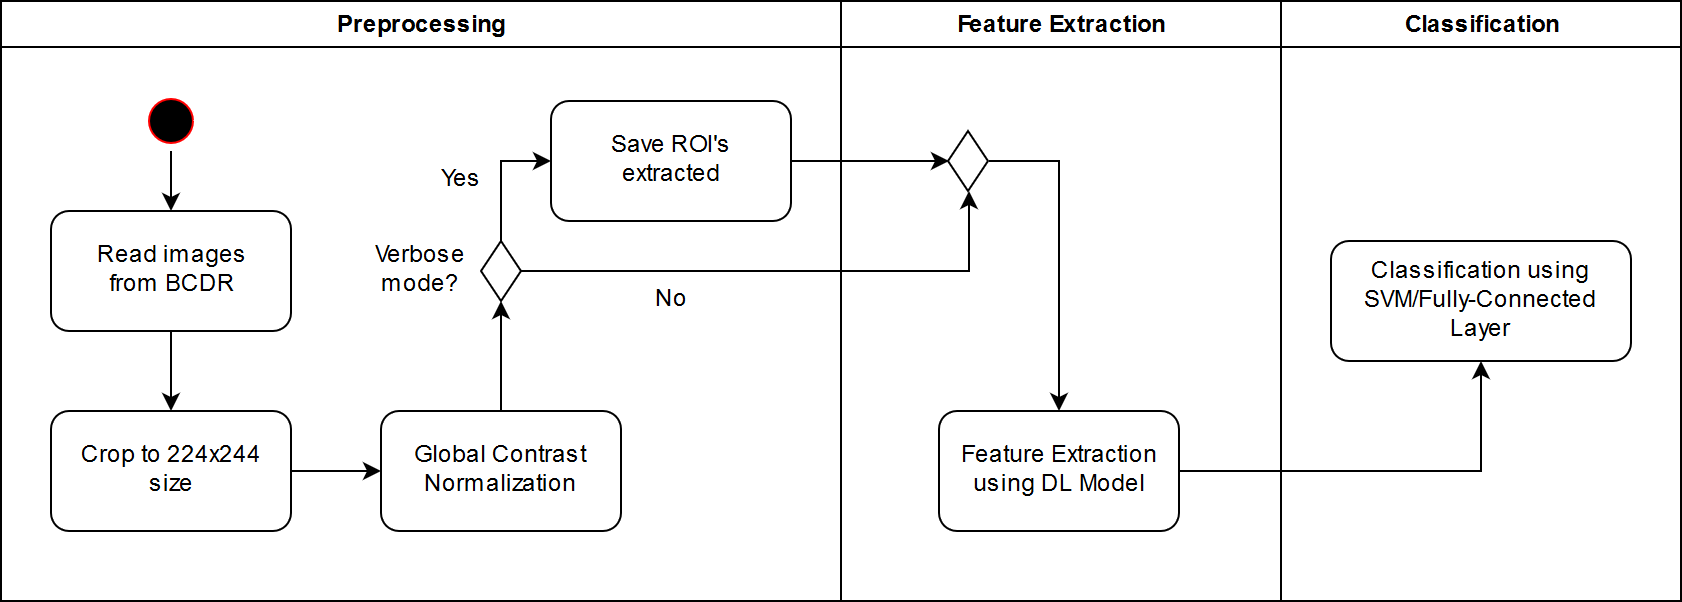
\includegraphics[width=\textwidth]{./img/workflow}
            \caption{System's main workflow}
            \label{fig:architecture}
          \end{figure}
        }

        \paragraph{Deep Learning Model}
          A Deep Learning model is a great tool to perform both feature extraction and classification processes, as referred before. So, a \gls{dl} model was developed to perform this tasks in our system. The model is based on Google's Inception V3 architecture \cite{szegedy2015rethinking}, which scheme can be seen on appendix \ref{appendix:inception-v3}. This architecture is an update to GoogLeNet, winner of the 2014 ImageNet contest, that has also been trained on the ImageNet dataset, where it achieved a top-1 accuracy (correct answer is the the prediction with the highest probability) of 78.0\% and a top-5 accuracy (correct answer is in the 5 predictions with higher probability) of 93.9\%. Since this architecture can score high accuracy values in the 1000 class ImageNet dataset, it can be fine-tuned to our 2 class dataset and, theoretically, achieve similar values of accuracy.

        \paragraph{Classifiers}
          After the feature extraction process, these can be used to represent an image in a simpler way. With this, a simpler classifier (\gls{svm}, \gls{mlp}, etc.) can be used to make a representation learning process. That is the main basis of neural networks: (i) feature learning in the hidden layers and (ii) classification of the features extracted using the output layer. The feature learning process gives a compressed representation of the input image, allowing us to reduce training times and to experiment different classifiers using the same features extracted using the \gls{dl} model. With the use of hand-crafted features alongside the features extracted with the \gls{dl} model, the performance can even increase, through the introduction of a human factor, since this set of features is extracted with the help of a medical professional.

    \section{Summary} \label{problem:summary}
      In this chapter the solution to the problem presented was detailed, presented some already existing solutions, alongside our proposed approach. Our approach follows an approach of feature classification, where these features are extracted using a Deep Learning model. Along with these features, there are included hand-crafted features, designed and extracted by experts, which adds the possibility of an improvement in performance/accuracy of the system. The following chapters will give the implementation details and the results obtained using our approach.

  % CHAPTER - Development -------------------------
  \chapter{Development} \label{development}
    This chapter presents details about the development phase of this dissertation. In general, the information presented focus on development details about the three phases of the system's workflow (preprocessing, feature extraction and classification) presented on section \ref{problem:proposal:architecture}. The following sections will present all the implementation details about the system developed.

    \begin{table}[t]
      \centering
      \begin{tabular}{ccc}
        \hline\\[-1em]
        & \textbf{CPU} & \textbf{GPU} \\\hline\\[-1em]
        Manufacturer & Intel\textsuperscript{\textregistered} & NVIDIA\textsuperscript{\textregistered} \\\hline\\[-1em]
        Model & i7-7700 & GeForce GTX 1080 \\\hline\\[-1em]
        \#Devices & 1 & 2 \\\hline\\[-1em]
        Release Date & Q1'17 & Q2'16 \\\hline\\[-1em]
        $\mu$Arch & Kaby Lake & Pascal \\\hline\\[-1em]
        \#Cores & 4 & 2560 \\\hline\\[-1em]
        Frequency & 3600 & 1607 \\\hline\\[-1em]
        L1 Cache & 2 x 32KB/core & 96KB/SM \\\hline\\[-1em]
        L2 Cache & 256KB/core & 4MB \\\hline\\[-1em]
        L3 Cache & 8MB & N/A \\\hline\\[-1em]
        Memory & 16GB (RAM) & 8GB \\\hline\\[-1em]
        Max Memory Bandwidth & 38.4GB/s & 320GB/s \\\hline\\[-1em]
      \end{tabular}
      \caption[Development system characteristics]{Development system's CPU\footnotemark\ and GPU's\footnotemark\ characteristics. This table presents the hardware that the systems used for the \gls{dl} model training possess. The use of 2 GPU's made possible a theoretical gain of 2x in the training time.}
      \label{tab:hw-details}
    \end{table}

    \section{Implementation} \label{development:implementation}

      This \gls{cadx} system was developed within a system which details are specified in table \ref{tab:hw-details} and all the code listings can be seen in the appendix \ref{listings}. This system allowed, with the use of 2 GPU's, to reduce training times of the Deep Learning models and all the classifiers. The system was developed using the Python language, because of its versatility and abundance of software libraries focused in the development of Deep Learning applications. The most well known libraries are:

      \begin{itemize}
          \item TensorFlow, developed by Google;
          \item Theano, developed by Université de Montréal;
          \item CogNitive TooKit, also known as CNTK, developed by Microsoft.
          \item Keras, an open source process that provides a high level wrapper to the libraries presented in the previous points.
      \end{itemize}

      For this system's implementation, the Keras library was selected, using TensorFlow backend, because of the simplicity of its API and the possibility of using highly optimized \gls{dl} APi's like TensorFlow in a quick and easy way. The possible gain of performance with the use of native TensorFlow was not considered as a factor, because it could not overcome the gain in development time.

      \subsection{The BCDR Dataset}

        \footnotetext{CPU details: \href{https://bit.ly/2uSSTlF}{https://bit.ly/2uSSTlF}}
        \footnotetext{GPU details: \href{https://bit.ly/2IwD5Hh}{https://bit.ly/2IwD5Hh}}

        The BCDR dataset \cite{lopez2012bcdr} is a benchmarking dataset that contains annotated images from mammographies (film and digital) from patients in the northern region of Portugal. This dataset studies that contain both biopsy proven \gls{mlo} and \gls{cc} views of the mammography. The lesions were mannualy segmented by medical experts at Centro Hospitalar São João and compiled in a CSV file that could be used to read and prepare the dataset by a computer program. Along with the outlines CSV, there is also a features CSV file, that contains a set of hand-crafted features that can also be used in classification processes. These features will be explored later on this document.

        % ...

        Having downloaded any of the BCDR instances (film or digital), we read the CSV into memory, that contains information like image filename, (x,y) outline points of the lesion and the classification (benign of malign). Python's libraries like \textit{csv} and \textit{Scikit-Image} were useful in this process.

      \subsection{Preprocessing}
        The preprocessing phase is a set of process that takes care of preparing the dataset images to be fed to feature extraction \gls{dl} model. This phase uses the \textit{OpenCV} and \textit{Scikit-Image} libraries to implement these processes. The processes include cropping of the images to fit the input shape of the \gls{dl} model, a data augmentation process and the application of filters to enhance features. The preprocessing pipeline can be seen in figure \ref{}.

        \paragraph{Cropping}
          The Inception V3 architecture, which was used for the development of the \gls{dl} model used in this system, requires that its input (the breast cancer images) has a resolution of 224x224. Having the (x,y) outline points, read from the outlines CSV file, we have the region were the lesion is located. With this, a 224x224 region is cropped arround the \gls{roi}. If the lesion is located is a region bigger than 224x224, it is zoom down to fit the 224x224 resolution.

        \paragraph{Data Augmentation}
          In order to increase the dataset's domain and quantity of information, data augmentation processes are used. In this system's partical case, the process used to increase the dataset's domais was the creation of new images by the use of a set of rotations (0, 90, 180 and 270 degrees), both in a normal and horizontally flipped image. This creates 7 new samples for each image, thereby increasing the size and variability of the dataset. This type of process can also prevent the overfitting process with the increase in the training domain.

        \paragraph{Filters for Feature Enhancement}
          In order to have a better feature learning process, the features to be learned need to be visible in order for the convolution filters to seize those features. Therefore, image filters are applied to enhance those features. In Arevalo et al. \cite{arevalo2016representation} approach, the filters applied were the global contrast normalization and the local contrast normalization. In our approach, just the global contrast normalization was applied, because of the lack of performance gain with the adition of a local contrast normalization.

          Global contrast normalization is a process used to normalize images exposed to different lightning conditions. This process subtracts the mean of the pixels in an image to every pixel. In formal terms, we can define the global contrast normalization as:

          \begin{equation}
            Y_{i,j}\ =\ X_{i,j}\ -\ \bar{x}
          \end{equation}

          where $X$ is the initial image, $\bar{x}$ represent the mean intensity of the pixels in image $X$, $r$ is the dimension of the image, in this case 224, and $Y$ is the resulting image. In our approach, we used a different approach, present by \cite{}, that garanties that the standard deviation accross all pixels is set to a constant $s$. In formal terms, our implementation (adapted to grayscale images) is defined by:

          \begin{equation}
            Y_{i,j}\ =\ s\ *\ \frac{X_{i,j}\ -\ \bar{x}}{max\ \begin{Bmatrix}
                      \ \epsilon,\ \sqrt{\lambda\ +\ \frac{1}{r^2}\sum_{i}\sum{j}\ (X_{i,j}\ -\ \bar{x})^2}\
                      \end{Bmatrix}}
          \end{equation}

          where $X$ is the initial image, $\bar{x}$ represent the mean intensity of the pixels in image $X$, $\lambda$ is a term to bias the standard deviation, and $Y$ is the resulting image. In this case, the denominator is constrained to be at least $\epsilon$. The Python code for this transformation can be seen in appendix \ref{listings:gcn}

      \subsection{Feature Extraction Model}
        % ...

        \paragraph{Train/Test Division}
          % ...

      \subsection{Classifiers}
        % ...

        \paragraph{Hand-Crafted Features}
          % ...

      \subsection{Performance Improving} \label{development:implementation:performance}
        % ...

    \section{Outcomes} \label{development:outcomes}
      % ...

    \section{Summary} \label{development:summary}
      % ...

  % CHAPTER - Application -------------------------
  \chapter{Case Studies / Experiments} \label{experiments}
    % ...

    \section{Experiment setup} \label{experiments:tests}
      % ...

    \section{Results} \label{experiments:results}
      % ...

    \section{Discussion} \label{experiments:discussion}
      % ...

    \section{Summary} \label{experiments:summary}
      % ...

  % CHAPTER - Conclusion/Future Work --------------
  \chapter{Conclusion} \label{conclusion}
    % ...

    \section{Conclusions} \label{conclusion:conclusions}
      % ...

    \section{Prospect for future work} \label{conclusion:future-work}
      % ...

  \bookmarksetup{startatroot} % Ends last part.

  \addtocontents{toc}{\bigskip} % Making the table of contents look good.
  %\null\newpage

  %- Bibliography (needs bibtex) -%
  \bibliography{dissertation}

  % Index of terms (needs  makeindex) -------------
  \printindex

	% APPENDIX ---------------------------------------
  \umappendix{Appendix}

    % Add appendix chapters
    \chapter{Support material} \label{support-material}
      \section{Inception V3 Architecture} \label{appendix:inception-v3}
        \begin{figure}[h]
          \centering
          \includegraphics[angle=90,width=0.32\textwidth]{"./img/inception-v3"}
          \caption[Inception V3 Architecture]{Inception V3 Architecture.}
        \end{figure}

    \chapter{Details of results} \label{results}
      Details of results whose length would compromise readability of main text; or

    \chapter{Listings} \label{listings}
      \section{Global Contrast Normalization implementation} \label{listings:gcn}
        \begin{lstlisting}[language=Python]
def global_contrast_normalization(X, s, lmda, epsilon):
    # Calculate mean of intensities
    X_average = np.mean(X)
    # Subtract mean to every pixel
    X = X - X_average
    # Final operation to make stddev equal to s
    contrast = np.sqrt(lmda + np.mean(X**2))
    X = s * X / max(contrast, epsilon)
    return X
        \end{lstlisting}

      \section{ZCA Whitening implementation} \label{listings:zca}
        \begin{lstlisting}
def zca_whitening(X):
    # Covariance matrix [column-wise variables]: Sigma = (X-mu)' * (X-mu) / N
    sigma = np.cov(X, rowvar=True) # [M x M]
    # Singular Value Decomposition. X = U * np.diag(S) * V
    U,S,V = np.linalg.svd(sigma)
        # U: [M x M] eigenvectors of sigma.
        # S: [M x 1] eigenvalues of sigma.
        # V: [M x M] transpose of U
    # Whitening constant: prevents division by zero
    epsilon = 1e-5
    # ZCA Whitening matrix: U * Lambda * U'
    ZCAMatrix = np.dot(U, np.dot(np.diag(1.0/np.sqrt(S + epsilon)), U.T)) # [M x M]
    X = np.dot(ZCAMatrix, X)
    return X
        \end{lstlisting}

    \chapter{Tooling} \label{tooling}
      \section{Dissertation Conceptual Map}
        \begin{figure}[h]
          \centering
          \includegraphics[angle=90,width=0.5\textwidth]{"./img/mind-map"}
          \caption[Dissertation Conceptual Map]{Dissertation Conceptual Map.}
          \label{appendix:concepts}
        \end{figure}

    %Anyone using \Latex\ should consider having a look at \TUG,
    %the \tug{\TeX\ Users Group}

  % Back Cover ------------------------------------
  %\umbackcover{
    % NB: place here information about funding, FCT project, etc in which the work is framed. Leave empty otherwise.
  %}

  \endgroup

\end{document}
